\documentclass[conference,10pt]{IEEEtran}
% SketchRAG final project report. Build: latexmk -pdf sketchrag.tex
% All numbers come from numbers.tex and tables/*.tex, generated from results/ by make_assets.py.
\usepackage[T1]{fontenc}
\usepackage{amsmath,amssymb}
\usepackage{graphicx}
\usepackage{booktabs}
\usepackage{xcolor}
\usepackage{algorithm}
\usepackage{algpseudocode}
\usepackage{tikz}
\usetikzlibrary{arrows.meta,positioning,fit}
\usepackage{cite}
\usepackage{url}
\usepackage[hidelinks]{hyperref}
\usepackage{microtype}
% generated by make_assets.py from results/; do not edit by hand
\newcommand{\GateScore}{41.7}
\newcommand{\FullScore}{38.1}
\newcommand{\BMScore}{46.0}
\newcommand{\DenseScore}{35.8}
\newcommand{\SketchScore}{29.9}
\newcommand{\RawScore}{42.5}
\newcommand{\AgentScore}{30.1}
\newcommand{\SaraScore}{38.2}
\newcommand{\AmberScore}{32.0}
\newcommand{\HybridScore}{38.3}
\newcommand{\GateTok}{1,213}
\newcommand{\FullTok}{14,232}
\newcommand{\RawTok}{1,549}
\newcommand{\GateTokPct}{8.5}
\newcommand{\GateLLMs}{5.8}
\newcommand{\FullLLMs}{61.5}
\newcommand{\AmberCalls}{3.0}
\newcommand{\GateHotKB}{454}
\newcommand{\DenseHotKB}{447}
\newcommand{\GateIngest}{25.6}
\newcommand{\KVSketch}{6.7}
\newcommand{\KVGate}{96.7}
\newcommand{\PKFull}{16.7}
\newcommand{\WQAGate}{33.3}
\newcommand{\WQASara}{51.9}
\newcommand{\WQAFull}{58.7}
\newcommand{\PRetBM}{70.0}
\newcommand{\PRetGate}{53.3}
\newcommand{\GovMin}{11.7}
\newcommand{\GovMax}{13.2}
\newcommand{\GainPct}{94}
\newcommand{\TokSavePct}{22}
\newcommand{\TruncatedFull}{105}
\newcommand{\NQ}{350}
\newcommand{\NFired}{190}
\newcommand{\NTrusted}{160}
\newcommand{\FiredPct}{54}
\newcommand{\FiredSketch}{30.0}
\newcommand{\FiredGate}{51.5}
\newcommand{\TrustedGate}{31.4}
\newcommand{\TrustedRaw}{32.2}
\newcommand{\FireKV}{100}
\newcommand{\FirePK}{93}
\newcommand{\FireGov}{0}
\newcommand{\AgentToolQ}{30}
\newcommand{\ResScore}{28.9}
\newcommand{\NoContig}{1.7}
\newcommand{\FrozenScore}{42.4}
\newcommand{\SweepMin}{40.3}
\newcommand{\SweepMax}{45.5}
\newcommand{\FbEight}{0.77}
\newcommand{\FbTwoFiftySix}{0.45}
\newcommand{\HotEight}{178}
\newcommand{\HotTwoFiftySix}{507}
\newcommand{\RecSketchEight}{0.28}
\newcommand{\RecSketchTwoFiftySix}{0.37}
\newcommand{\FrozenRerun}{43.3}
\newcommand{\CmsMin}{40.0}
\newcommand{\CmsMax}{43.3}
\newcommand{\CmsFbSixtyFour}{0.75}
\newcommand{\CmsFbFiveTwelve}{0.51}
\newcommand{\CmsHotTwoK}{1,023}
\newcommand{\CmsHotFiveTwelve}{416}
\newcommand{\StressWords}{8,488,204}
\newcommand{\StressMWords}{8.5}
\newcommand{\StressChunks}{65,127}
\newcommand{\StressHotSixtyFour}{1.0}
\newcommand{\StressHotTwoFiftySix}{3.7}
\newcommand{\StressDense}{146}
\newcommand{\StressText}{50}
\newcommand{\StressIngest}{4.5}
\newcommand{\RecDense}{0.44}
\newcommand{\RecBM}{0.38}
\newcommand{\RecSRSketch}{0.12}
\newcommand{\RecSRGate}{0.23}
\newcommand{\RecSRRaw}{0.24}
\newcommand{\StressDocs}{1,115}
\newcommand{\DemoGate}{27}
\newcommand{\DemoDense}{25}
\newcommand{\DemoQ}{56}
\newcommand{\StressFb}{1.00}
\newcommand{\StressProbes}{100}
\newcommand{\EMGate}{34.8}
\newcommand{\EMLLM}{34.5}
\newcommand{\EMFull}{37.7}
\newcommand{\EMQ}{120}
\newcommand{\EMTasks}{6}
\newcommand{\CellKBMax}{14.2}
\newcommand{\CellKBMean}{10.4}

\newcommand{\sys}[1]{\textsc{#1}}
\renewcommand{\algorithmicrequire}{\textbf{Input:}}
\renewcommand{\algorithmicensure}{\textbf{Output:}}

\begin{document}

\title{SketchRAG: Approximate Streaming Summaries as Retrieval Context for Agentic AI}

\author{
\IEEEauthorblockN{R Ranjith Kumar}
\IEEEauthorblockA{2023BCD0030\\IIIT Kottayam}
\and
\IEEEauthorblockN{Bhuvan S M}
\IEEEauthorblockA{2023BCS0198\\IIIT Kottayam}
\and
\IEEEauthorblockN{Hariprashanth M}
\IEEEauthorblockA{2023BCS0036\\IIIT Kottayam}
\and
\IEEEauthorblockN{Nooh K}
\IEEEauthorblockA{2023BCD0003\\IIIT Kottayam}
}

\maketitle

\begin{abstract}
Agents that read continuous streams cannot afford to keep and search every chunk forever. We present SketchRAG, which
maintains a bounded, query-independent summary of a text stream---semantic cells with extractive digests, per-cell
Count-Min Sketches, Misra--Gries heavy hitters and streaming IDF, all updated in one pass---and uses it as the
retrieval layer. Its key component is an \emph{error-bound gate}: the Count-Min guarantee, checked against each cell's
digest, decides when the summary cannot be trusted and raw evidence must be read from cold storage. On \NQ{}
LongBench and $\infty$-Bench questions answered by qwen2.5:7b-instruct, the gated system scores \GateScore{}, ahead of
full context (\FullScore{}), dense RAG (\DenseScore{}), SARA-lite (\SaraScore{}) and AMBER-lite (\AmberScore{}), while
sending the fewest LLM context tokens of any system (\GateTok{} per question, \GateTokPct\% of full context). BM25 RAG
remains the strongest system (\BMScore{}). The gate is calibrated: on the \FiredPct\% of questions it escalates, raw
evidence lifts the score from \FiredSketch{} to \FiredGate{}, while on the questions it trusts, always reading raw text
would add under one point. With a shared base model, SketchRAG matches the official EM-LLM implementation (\EMGate{}
vs.\ \EMLLM{}). On an \StressMWords{}M-word stream, hot memory stays at \StressHotSixtyFour{}--\StressHotTwoFiftySix{}~MB
against a \StressDense{}~MB dense index, but answer recall falls (\RecSRGate{} vs.\ \RecDense{}), which is the main
limitation we report.
\end{abstract}

\begin{IEEEkeywords}
retrieval-augmented generation, data streams, Count-Min Sketch, LLM agents, long context, memory
\end{IEEEkeywords}

\section{Introduction}
Large language model (LLM) agents increasingly work over information that arrives continuously: logs, transcripts,
reports and documents appended over time. Two families of methods give such an agent access to its history.
Retrieval-augmented generation (RAG)~\cite{lewis2020rag} keeps every chunk and a vector for each one, so its searchable
index grows linearly with the stream. Long-context and episodic-memory methods such as EM-LLM~\cite{fountas2025emllm}
avoid retrieval over text but keep per-event key/value state for the whole history and need access to model
internals. Simply placing everything in the prompt is costly and brittle: models lose information in the middle of
long inputs~\cite{liu2024lost}, and documents longer than the window must be truncated.

The data-stream literature offers a different tool: \emph{synopses} that summarise an unbounded stream in bounded
memory with provable error~\cite{muthukrishnan2005streams}. This project asks whether such synopses can serve as the
retrieval layer of an agent. Our central research question is: \emph{can approximate streaming summaries provide a
memory-efficient retrieval context for agentic AI while keeping answer quality comparable to full-context and RAG
approaches?} We study it through five sub-questions: whether the summaries preserve enough information (RQ1), how the
approach compares with episodic-memory, adaptive-memory and compression methods (RQ2), how the memory budget affects
accuracy (RQ3), whether the system can decide when the summary is insufficient (RQ4), and which trade-off between
memory, compression, latency and accuracy is best (RQ5).

\textbf{Contributions.} (i) SketchRAG, a single-pass streaming memory that combines streaming clustering, per-cell
Count-Min Sketches~\cite{cormode2005countmin}, Misra--Gries heavy hitters~\cite{misra1982repeated} and extractive
digests, maintained \emph{before} any query and bounded in size regardless of stream length. (ii) An error-bound gate
that turns the Count-Min guarantee into a per-cell, per-query signal for whether the summary can be trusted, with
raw evidence fetched from cold storage only for escalated cells. (iii) An evaluation on \NQ{} test questions over 12
tasks against full context, BM25 and dense RAG, re-implementations of SARA~\cite{jin2026sara} and
AMBER~\cite{qin2025amber}, a reproduction of EM-LLM from its official code, ablations, memory-budget sweeps and an
\StressMWords{}M-word stress test, all run with open models served by Ollama~\cite{ollama}.

\section{Related Work}
\textbf{Episodic memory.} EM-LLM~\cite{fountas2025emllm} segments the token stream into events at points of high
surprise, stores each event's key/value cache, and at inference retrieves similar events plus temporally contiguous
neighbours. It scales to very long inputs without fine-tuning, but its memory grows with the input and it needs the
model's internals and a large GPU. Our cells play the role of events and our temporal-neighbour rule follows its
contiguity buffer, but we operate on text and keep a fixed budget.

\textbf{Adaptive and agentic memory.} AMBER~\cite{qin2025amber} builds a memory note during each question with several
LLM roles: a memory updater, an adaptive collector that decides whether to retrieve again, and a multi-granular
filter. MemGPT~\cite{packer2023memgpt} lets the LLM page information in and out of its context. Both put the LLM in
charge of memory decisions, which costs extra calls; we test this choice directly (an LLM-driven variant of
SketchRAG) and find that a deterministic sketch signal is better calibrated.

\textbf{Context compression.} SARA~\cite{jin2026sara} retrieves generously and compresses the retrieved evidence to a
fixed budget, mixing natural-language snippets with learned compression vectors. Compression happens \emph{after} a
query. SketchRAG compresses the \emph{stream} continuously, before any query arrives.

\textbf{Streaming synopses.} The Count-Min Sketch~\cite{cormode2005countmin} estimates item frequencies in
$O(\frac{1}{\varepsilon}\log\frac{1}{\delta})$ space, never under-counting and over-counting by at most $\varepsilon N$
with probability $1-\delta$. Misra--Gries~\cite{misra1982repeated} keeps every item with frequency above
$N/(k{+}1)$ using $k$ counters, and reservoir sampling~\cite{vitter1985reservoir} keeps a uniform fixed-size sample.
Clustering features~\cite{zhang1996birch} and merge-and-reduce~\cite{guha2003clustering} cluster streams in bounded
memory. To our knowledge, these synopses have not been used as the retrieval layer of an LLM agent, nor has a sketch's
error bound been used to decide when to read raw evidence.

\section{Preliminaries: Streaming Synopses}
We use the cash-register stream model~\cite{muthukrishnan2005streams}: items (here, terms of arriving chunks) arrive
one at a time, each update must be processed in small time and space, and $N$ denotes the total count seen so far.

\textbf{Count-Min Sketch.} A Count-Min Sketch~\cite{cormode2005countmin} is a $d\times w$ table of counters with $d$
pairwise-independent hash functions $h_1,\dots,h_d$. An update of item $x$ increments $C[j,h_j(x)]$ for every row $j$,
and a query returns $\hat f(x)=\min_j C[j,h_j(x)]$. With $w=\lceil e/\varepsilon\rceil$ and $d=\lceil\ln(1/\delta)\rceil$,
\begin{equation}
f(x)\;\le\;\hat f(x)\;\le\;f(x)+\varepsilon N \quad\text{with probability}\ \ge 1-\delta .
\label{eq:cms}
\end{equation}
Our cells use $w{=}512$ and $d{=}3$, so $\varepsilon\approx0.0053$ and $\delta\approx0.05$. We use the
\emph{conservative update}, which raises only the counters that equal the current minimum; it keeps the guarantee and
reduces over-counting. The sketch is linear: the table of a union of two streams is the sum of their tables. The gate
uses two thresholds derived from it: the expected collision mass of one row, $\nu=N/w$ (a tight but non-guaranteed
noise floor), and the guaranteed bound $\varepsilon N$ of~\eqref{eq:cms}.

\textbf{Misra--Gries.} With $k$ counters, Misra--Gries~\cite{misra1982repeated} keeps a candidate set of heavy items;
when a new item finds no free counter, all counters are decremented. Every item with frequency above $N/(k{+}1)$
survives, and each estimate is at most $N/(k{+}1)$ below the truth. We use $k{=}256$ to expose the stream's topics.

\textbf{Streaming IDF.} A second, global Count-Min Sketch counts the number of chunks containing each term, giving a
document frequency $\widehat{df}(t)$ and $\mathrm{idf}(t)=\log\frac{n+1}{\widehat{df}(t)+1}+1$ after $n$ chunks. Because the
sketch over-counts, the IDF it yields is a conservative (low) estimate, so a term that looks rare really is rare.

\section{Method}
\begin{figure*}[t]
\centering
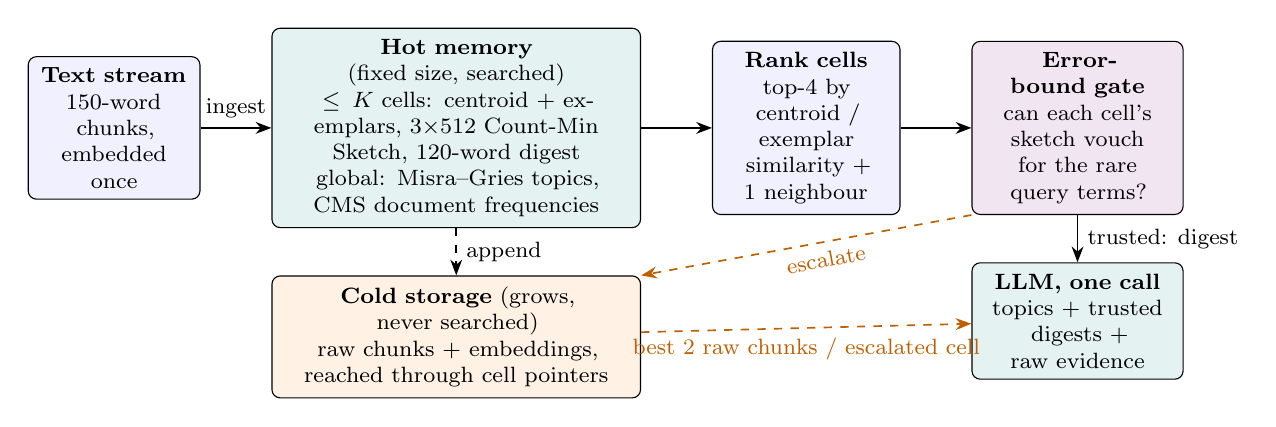
\begin{tikzpicture}[font=\footnotesize, node distance=6mm and 9mm,
  box/.style={draw, rounded corners=3pt, align=center, inner sep=4pt, minimum height=11mm},
  arr/.style={-{Stealth[length=2mm]}, semithick}, esc/.style={arr, dashed, orange!75!black}]
\node[box, fill=blue!6, text width=19mm] (stream) {\textbf{Text stream}\\150-word chunks,\\embedded once};
\node[box, fill=teal!10, right=of stream, text width=44mm] (hot) {\textbf{Hot memory} (fixed size, searched)\\
$\le K$ cells: centroid + exemplars, $3{\times}512$ Count-Min Sketch, 120-word digest\\
global: Misra--Gries topics, CMS document frequencies};
\node[box, fill=blue!6, right=of hot, text width=21mm] (rank) {\textbf{Rank cells}\\top-4 by centroid / exemplar similarity + 1 neighbour};
\node[box, fill=violet!10, right=of rank, text width=24mm] (gate) {\textbf{Error-bound gate}\\can each cell's sketch vouch for the rare query terms?};
\node[box, fill=orange!10, below=of hot, text width=44mm] (cold) {\textbf{Cold storage} (grows, never searched)\\raw chunks + embeddings, reached through cell pointers};
\node[box, fill=teal!10, below=of gate, text width=24mm] (llm) {\textbf{LLM, one call}\\topics + trusted digests + raw evidence};
\draw[arr] (stream) -- node[above] {ingest} (hot);
\draw[arr, dashed] (hot) -- node[right] {append} (cold);
\draw[arr] (hot) -- (rank);
\draw[arr] (rank) -- (gate);
\draw[arr] (gate) -- node[right] {trusted: digest} (llm);
\draw[esc] (gate.south west) -- node[below, sloped, pos=0.45] {escalate} (cold.north east);
\draw[esc] (cold) -- node[below] {best 2 raw chunks / escalated cell} (llm);
\end{tikzpicture}
\caption{SketchRAG. Each chunk updates a fixed-size hot memory in one pass and is appended to cold storage. At query
time cells are ranked, and the gate escalates only the cells whose Count-Min Sketch cannot vouch for their digest; their
raw chunks replace the digest in the LLM's context.}
\label{fig:arch}
\end{figure*}

Fig.~\ref{fig:arch} gives an overview. A document or stream is split into chunks of about 150 word units (long machine
tokens such as UUIDs are charged per six characters so that a chunk holds a similar number of LLM tokens). Each chunk
is embedded once with bge-small-en-v1.5~\cite{xiao2023cpack} and passed to the memory, which updates two stores.

\subsection{Hot memory}
The hot memory is the only part searched at query time and its size is fixed by the configuration.

\textbf{Semantic cells.} Each cell is a clustering feature~\cite{zhang1996birch}: the sum $\mathbf{s}$ and count $n$ of its
member embeddings, from which the centroid $\mathbf{s}/\lVert\mathbf{s}\rVert$ and radius follow (for unit vectors
$\mathbb{E}\lVert x-\mu\rVert^2 = 1-\lVert\mu\rVert^2$, $\mu=\mathbf{s}/n$), plus the span of stream positions it covers.
A chunk joins the most similar cell if cosine similarity is at least 0.90 (with a small bonus for the current cell,
following EM-LLM's event continuity); otherwise it opens a new cell. When the number of cells exceeds the budget $K$,
the pair with the smallest Ward cost~\cite{ward1963hierarchical} $\frac{n_a n_b}{n_a+n_b}\lVert\mu_a-\mu_b\rVert^2$ is
merged (merge-and-reduce~\cite{guha2003clustering}). Ward linkage resists a single cell absorbing the whole stream.

\textbf{Per-cell Count-Min Sketch.} Each cell counts its content terms in a $3\times512$ sketch with conservative update.
Because the sketch is linear, merging two cells adds their tables, so the guarantee survives merges.

\textbf{Digest and exemplars.} Each cell keeps an extractive digest of at most 120 words: the most salient sentences,
scored by the mean streaming IDF of their terms and by how typical their chunk is of the cell. No LLM is called at
ingest time. A cell also keeps up to eight diverse member embeddings (exemplars), selected by repeatedly dropping the
most redundant one; they play the role of EM-LLM's representative tokens when cells are ranked.

\textbf{Global synopses.} A Count-Min Sketch of document frequencies gives a streaming IDF, and a Misra--Gries table of
the 256 heaviest terms gives the stream's topics, shown to the LLM as global context.

\subsection{Memory and time complexity}
\begin{table}[t]
\centering
\caption{Hot-memory accounting, measured on a 194-chunk NarrativeQA stream with $K{=}64$ cells (total 762~KB). Cold storage is not included.}
\label{tab:memory}
\setlength{\tabcolsep}{4pt}
\begin{tabular}{lrl}
\toprule
Component & Bytes & Scope \\
\midrule
Centroid sum (384 $\times$ fp32) & 1{,}536 & per cell \\
Count-Min Sketch ($3\times512$ int32) & 6{,}144 & per cell \\
Exemplars ($\le$8 $\times$ 384 fp16; mean here) & 2{,}244 & per cell \\
Extractive digest ($\le$120 words; mean) & 669 & per cell \\
Document-frequency CMS ($3\times8192$) & 98{,}304 & global \\
Misra--Gries table ($k{=}256$) & 2{,}492 & global \\
\bottomrule
\end{tabular}
\end{table}
Table~\ref{tab:memory} accounts for the hot memory. A cell occupies \CellKBMean{}~KB on average and at most
\CellKBMax{}~KB, dominated by its sketch and exemplars, plus about 100~KB of global synopses; a 64-cell memory is
therefore about 1~MB however long the stream is. Ingesting a chunk costs $O(Kd)$ to score the $K$ cells against the
$d{=}384$-dimensional embedding, $O(L)$ sketch updates for its $L$ terms, and, when the budget is exceeded, an $O(K^2 d)$
Ward merge (we recompute the pairwise cost matrix; at $K\le256$ this takes milliseconds). Answering costs $O(K E d)$ to
rank cells with $E\le 8$ exemplars each, $O(|R|)$ sketch queries per retrieved cell for the gate, and, for escalated
cells only, a scan of that cell's pointer list in cold storage.

\subsection{Cold storage}
Every raw chunk, its embedding and the cell$\rightarrow$chunk pointer lists are appended to cold storage, which is never
searched and is read only when the gate escalates a cell. Cold storage grows with the stream; we report hot and cold
sizes separately and never describe the system as bounded end to end.

\subsection{Query time and the error-bound gate}
A question is embedded and each cell is scored by the maximum cosine similarity over its centroid and exemplars. The
top four cells are kept, plus the temporal neighbour of the best cell (EM-LLM's contiguity). The gate
(Algorithm~\ref{alg:gate}) then examines the \emph{rare} query terms, those with streaming IDF at least 2.5.

\begin{algorithm}[t]
\caption{Error-bound gate for one query}\label{alg:gate}
\begin{algorithmic}[1]
\Require retrieved cells $C$, rare query terms $R$
\Ensure cells $E\subseteq C$ escalated to raw evidence
\State $E\gets\emptyset$; $\mathit{conf}\gets\mathbf{false}$
\For{$c\in C$}
  \If{$\mathrm{radius}(c)>0.75$} \Comment{\emph{loose}}
    \State $E\gets E\cup\{c\}$
  \EndIf
  \For{$t\in R$}
    \State $\hat f\gets \mathrm{CMS}_c(t)$;\; $\nu\gets N_c/w$
    \If{$\hat f>\varepsilon N_c$} $\mathit{conf}\gets\mathbf{true}$ \EndIf
    \If{$\hat f-\nu\ge1 \wedge t\notin\mathrm{dig}(c)$} \Comment{\emph{lossy}}
      \State $E\gets E\cup\{c\}$
    \EndIf
  \EndFor
\EndFor
\If{$R\neq\emptyset \wedge \neg\mathit{conf}$} \Comment{\emph{unresolved}}
  \State $E\gets E\cup\mathrm{top}_2(C)$
\EndIf
\State \Return $E$
\end{algorithmic}
\end{algorithm}

A cell is escalated when it is \emph{lossy} (the sketch places a rare term in the cell above its noise floor $N/w$, but
the digest lacks it, so the summary dropped the fact; we also require some digest sentence to hold two rare terms
together), \emph{loose} (its radius exceeds 0.75, so its digest averages too much), or \emph{unresolved} (no retrieved
cell holds any rare term above the guaranteed bound $\varepsilon N$, so the sketch cannot locate the answer and the top
two cells are read). Questions without rare terms, such as summarisation requests, are answered from the digests.
For each escalated cell, its cold chunks are re-ranked by cosine similarity plus IDF-weighted term overlap and the best
two replace the cell's digest. The LLM is called once with the heavy-hitter topics, the trusted digests and the raw
evidence.

\textbf{Policies.} We compare five SketchRAG policies: \sys{sketch} (digests only), \sys{raw} (escalate every retrieved
cell), \sys{gate} (Algorithm~\ref{alg:gate}), \sys{agent} (the LLM sees the digests and may call
\texttt{fetch\_raw}/\texttt{search\_memory} tools for up to three rounds) and \sys{hybrid} (the gated context plus the
same tools).

\section{Implementation}
SketchRAG is implemented from scratch in Python and NumPy: the Count-Min Sketch, Misra--Gries, reservoir sampling,
streaming clustering and the gate are our own code, because SciPy and scikit-learn were blocked on our development
machine. Unit tests check on synthetic Zipf streams that the Count-Min bound~\eqref{eq:cms} holds, survives merging and is
tightened by conservative update, that Misra--Gries keeps its guarantee, that reservoir samples are uniform, and that
hot memory stays bounded while cold storage grows; all 12 pass. Every
system implements one interface that turns a question and its document stream into an LLM context, and a single runner
calls the LLM with the same prompt for all of them. Chunk embeddings are computed once on a GPU and cached in a
content-addressed SQLite store, so every system and every run sees identical vectors.

All LLM calls go through Ollama~\cite{ollama}, which lets the same code run against a local CPU server during
development and against a GPU server inside Kaggle notebooks for the bulk runs. The runner is resumable and writes one
JSON record per (system, question), so a crashed notebook loses no finished questions; the full set of runs took about
6.4~GPU-hours for the main comparison and 1.3 for ablations and sweeps. Every table and figure in this report is
regenerated from these records by a script, and every number in the text is a macro produced by the same script.

\section{Experimental Setup}
\textbf{Data.} The test split is a fixed-seed sample (seed 0) of 30 questions from each of nine English LongBench
tasks~\cite{bai2024longbench} (NarrativeQA, Qasper, MultiFieldQA, HotpotQA, 2WikiMQA, MuSiQue, GovReport, QMSum,
PassageRetrieval) and two $\infty$-Bench retrieval tasks~\cite{zhang2024infinitebench} (PassKey, KV), plus 20 En.QA
questions over books of about 190K tokens: \NQ{} questions in total. Each document is fed to every system as a chunk
stream. All settings were tuned on a disjoint development split (seed 1000, 10 questions per task); the test split was
frozen before tuning. The \emph{stress test} concatenates every English LongBench QA and summary document (\StressDocs{}
documents, \StressWords{} words, \StressChunks{} chunks) into one stream in a fixed shuffled order and asks
\StressProbes{} probe questions whose source documents are spread evenly over it.

\textbf{LLM.} Every system uses qwen2.5:7b-instruct~\cite{qwen2025qwen25} served by Ollama on a Kaggle T4 GPU, with a
32,768-token window, greedy decoding, a fixed seed and the same prompt template; only the context differs. Full context
is middle-truncated to the window following LongBench (\TruncatedFull{} of its \NQ{} prompts needed truncation).

\textbf{Baselines.} \emph{Full context}; \emph{BM25 RAG}~\cite{robertson2009bm25} (top-5 chunks); \emph{dense RAG}
(FAISS~\cite{johnson2021faiss} inner product over the same bge embeddings, top-5); \emph{SARA-lite} (dense top-20,
compressed to a 600-word budget by sentence selection; SARA's learned compression vectors are not reproduced);
\emph{AMBER-lite} (up to three rounds in which the LLM updates a memory note, decides whether to retrieve again and
filters sentences; AMBER's trained filters are not reproduced); and \emph{EM-LLM} from its official repository with
its Phi-3.5-mini~\cite{abdin2024phi3} configuration on two Kaggle T4 GPUs. For a like-for-like comparison, SketchRAG and
the RAG baselines are rerun on the same question subset with the same base model (phi3.5 through Ollama).

\textbf{Metrics.} Answer quality uses LongBench's official metrics: token F1 for QA, ROUGE-L for summaries, accuracy for
passage retrieval and exact containment for PassKey and KV; scores are averaged per task and then over tasks.
Retrieval quality is \emph{answer recall}, whether a gold answer string appears in the context sent to the LLM, a
proxy because the benchmarks lack evidence annotations. Efficiency is measured as LLM context tokens and calls per
question, LLM time, hot-memory bytes, ingest time per chunk and the gate's fallback rate.

\section{Results}
\begin{table*}[t]
\centering
\caption{Answer quality on the 350 test questions (task score $\times$100; F1 for QA, ROUGE-L for GovR/QMS, accuracy for PRet/PKey/KV). All systems use qwen2.5:7b-instruct with the same prompt; only the context differs. Best per column in bold.}
\label{tab:main}
\setlength{\tabcolsep}{4.2pt}
\begin{tabular}{lrrrrrrrrrrrrr}
\toprule
System & NQA & Qasp & MFQA & HQA & 2WQA & MuSQ & GovR & QMS & PRet & PKey & KV & EnQA & \textbf{Avg} \\
\midrule
Full context & \textbf{26.8} & 51.4 & 51.7 & \textbf{65.6} & \textbf{58.7} & 24.2 & \textbf{15.9} & 19.4 & \textbf{93.3} & 16.7 & 10.0 & 23.0 & 38.1 \\
BM25 RAG & 18.7 & 45.8 & 47.5 & 51.4 & 38.0 & 17.6 & 11.7 & \textbf{20.6} & 70.0 & \textbf{100.0} & \textbf{96.7} & \textbf{34.3} & \textbf{46.0} \\
Dense RAG & 14.7 & 38.8 & 51.4 & 47.2 & 38.3 & 27.4 & 11.7 & 20.0 & 50.0 & \textbf{100.0} & 6.7 & 23.5 & 35.8 \\
SARA-lite & 17.2 & \textbf{53.5} & \textbf{55.0} & 61.4 & 51.9 & \textbf{33.5} & 12.0 & 18.8 & 16.7 & \textbf{100.0} & 16.7 & 22.0 & 38.2 \\
AMBER-lite & 11.1 & 42.6 & 53.3 & 44.8 & 43.1 & 32.9 & 9.9 & 18.9 & 0.0 & \textbf{100.0} & 10.0 & 18.0 & 32.0 \\
\midrule
SketchRAG-sketch & 13.2 & 24.1 & 36.5 & 39.9 & 28.3 & 18.6 & 11.8 & 17.5 & 46.7 & \textbf{100.0} & 6.7 & 16.0 & 29.9 \\
SketchRAG-raw & 20.3 & 38.6 & 50.7 & 52.8 & 28.5 & 18.8 & 13.2 & 19.4 & 53.3 & \textbf{100.0} & \textbf{96.7} & 17.5 & 42.5 \\
SketchRAG-gate & 15.0 & 36.2 & 44.0 & 50.2 & 33.3 & 21.9 & 11.7 & 18.9 & 53.3 & \textbf{100.0} & \textbf{96.7} & 19.0 & 41.7 \\
SketchRAG-agent & 8.9 & 20.5 & 36.0 & 32.8 & 20.6 & 12.3 & 12.3 & 18.1 & 30.0 & \textbf{100.0} & 60.0 & 10.0 & 30.1 \\
SketchRAG-hybrid & 14.3 & 33.1 & 41.8 & 47.5 & 22.6 & 17.9 & 12.4 & 18.7 & 40.0 & \textbf{100.0} & 93.3 & 17.6 & 38.3 \\
\bottomrule
\end{tabular}
\end{table*}

\subsection{Answer quality and cost (RQ1, RQ2, RQ5)}
Table~\ref{tab:main} gives per-task scores and Table~\ref{tab:eff} the costs. SketchRAG-gate scores \GateScore{},
ahead of full context (\FullScore{}), SARA-lite (\SaraScore{}), dense RAG (\DenseScore{}) and AMBER-lite
(\AmberScore{}), while sending \GateTok{} context tokens per question, the fewest of any system and \GateTokPct\% of
full context, with one LLM call and \GateLLMs{}~s of LLM time against \FullLLMs{}~s for full context
(Fig.~\ref{fig:pareto}). Plain BM25 RAG is the strongest system (\BMScore{}), mainly through exact-match tasks: on
PassageRetrieval it scores \PRetBM{} against \PRetGate{}. Full context fails PassKey (\PKFull{}) because middle
truncation removes the needle.

The summary alone is not enough (RQ1): \sys{sketch} scores \SketchScore{}, losing most on questions that need an exact
string; on $\infty$-Bench KV it scores \KVSketch{} and the gate lifts this to \KVGate{}. On global questions the summary
suffices: GovReport has no rare query terms, the gate never fires (\FireGov\%) and all three policies score
\GovMin{}--\GovMax{}. SketchRAG trails on multi-hop QA, where evidence is spread over more chunks than five cells hold:
on 2WikiMQA the gate scores \WQAGate{} against \WQASara{} (SARA-lite) and \WQAFull{} (full context).

\begin{table}[t]
\centering
\caption{Efficiency per question (means over 350 questions). Tok = LLM context tokens; Rec = answer recall of the context (gold string present); Fb = gate fallback rate.}
\label{tab:eff}
\setlength{\tabcolsep}{3.4pt}
\begin{tabular}{lrrrrr}
\toprule
System & Tok & Calls & LLM s & Rec & Fb \\
\midrule
Full context & 14{,}232 & 1.00 & 61.5 & 0.51 & 0.00 \\
BM25 RAG & 1{,}327 & 1.00 & 8.1 & 0.49 & 0.00 \\
Dense RAG & 1{,}361 & 1.00 & 6.9 & 0.41 & 0.00 \\
SARA-lite & 2{,}435 & 1.00 & 12.9 & 0.45 & 0.00 \\
AMBER-lite & 2{,}223 & 2.97 & 31.8 & 0.33 & 0.00 \\
SketchRAG-sketch & 1{,}284 & 1.00 & 6.1 & 0.35 & 0.00 \\
SketchRAG-raw & 1{,}549 & 1.00 & 7.6 & 0.50 & 1.00 \\
SketchRAG-gate & 1{,}213 & 1.00 & 5.8 & 0.46 & 0.54 \\
SketchRAG-agent & 2{,}727 & 1.16 & 9.4 & 0.40 & 0.06 \\
SketchRAG-hybrid & 1{,}553 & 1.02 & 6.3 & 0.46 & 0.55 \\
\bottomrule
\end{tabular}
\end{table}

\begin{figure}[t]
\centering
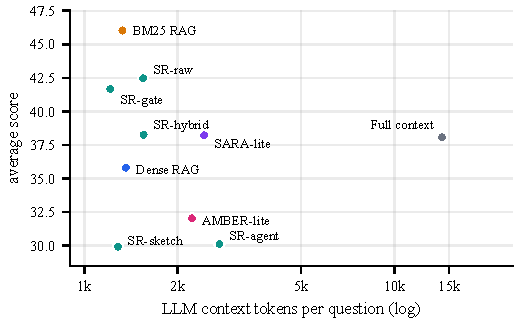
\includegraphics[width=\columnwidth]{figs/pareto.pdf}
\caption{Answer quality vs.\ LLM context tokens (log scale). SketchRAG-gate (SR-gate) has the cheapest context of any
system and the third-best score.}
\label{fig:pareto}
\end{figure}

\subsection{Is the gate calibrated? (RQ4)}
The gate escalates \NFired{} of the \NQ{} questions (\FiredPct\%). On those, raw evidence lifts the score from
\FiredSketch{} (digest only) to \FiredGate{}. On the \NTrusted{} questions it trusts, always reading raw text would have
moved the score only from \TrustedGate{} to \TrustedRaw{}. It fires on \FireKV\% of KV and \FirePK\% of PassKey
questions, where digests drop exact keys, and never on GovReport. Overall it recovers \GainPct\% of the gain of always
reading raw evidence while sending \TokSavePct\% fewer tokens than \sys{raw}. Fig.~\ref{fig:fire} shows the fire
rate per task: it follows how much each task depends on exact strings.

\begin{figure}[t]
\centering
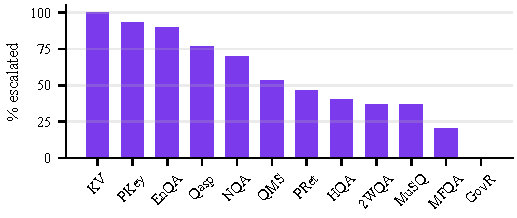
\includegraphics[width=\columnwidth]{figs/fire_rate.pdf}
\caption{Share of questions the gate escalates, per task. Exact-key tasks (KV, PassKey) almost always escalate;
summarisation (GovR) never does.}
\label{fig:fire}
\end{figure}

\begin{table*}[t]
\centering
\caption{Real answers from the main run (qwen2.5:7b). The gate's escalation reason is shown per question. The last row is a failure: the gate escalated, but the evidence was not in the retrieved cells.}
\label{tab:cases}
\footnotesize
\setlength{\tabcolsep}{3.5pt}
\begin{tabular}{l p{4.0cm} l l l l l}
\toprule
Task & Question (abridged) & Gold & Digest only & SketchRAG-gate & Full context & Gate \\
\midrule
NQA & Who did Baron Conrad kill? &Baron Frederick & not enough informa\ldots & Baron Frederick & Baron Henry & unresolved \\
KV & Value for key 35b9fdc1-c2c2-\ldots? &e2e6376e-5c57-4\ldots & 14f1 & e2e6376e-5c57-4b42\ldots & b7000000-202d-4b0b\ldots & unresolved \\
MuSQ & What is the place of birth of who does the voice of stan on the series that Insecurity is\ldots &Denver & Malcolm McDowell & Denver & Trey Parker & lossy \\
2WQA & Who is younger, Peter Rosegger or Ruel Redinger? &Ruel Redinger & Peter Rosegger & Peter Rosegger & Ruel Redinger & unresolved \\
\bottomrule
\end{tabular}
\end{table*}
Table~\ref{tab:cases} shows real answers. In the NarrativeQA question the digest alone makes the model answer
``not enough information''; the gate finds no cell that can vouch for the rare name, reads two cells raw, and the model
names the victim, while full context, whose prompt was truncated, names the wrong baron. For the KV key no summary can
hold a UUID, and only the raw chunk recovers the value. In the MuSiQue question the sketch places the rare terms in a cell
whose digest dropped them (\emph{lossy}), and the raw text supplies the answer. The 2WikiMQA row is a failure typical of
multi-hop questions: the gate escalates, but the evidence for the second entity lies in cells that were never
retrieved, so reading raw text cannot help.

Leaving the decision to the LLM does not work at this scale: the \sys{agent} policy called a tool on only \AgentToolQ{}
of \NQ{} questions, mostly KV, and scored \AgentScore{}, close to digests alone. \sys{Hybrid} (\HybridScore) adds
tokens and scores below the gate alone, most likely because extra tool output distracts the 7B model. The calibrated
signal therefore comes from the sketch's error bound, not from the model's self-assessment.

\subsection{Ablations and memory budget (RQ3, RQ5)}
\begin{table}[t]
\centering
\caption{Ablations of SketchRAG-gate (110 questions, 11 tasks $\times$ 10). $\Delta$ is relative to the frozen configuration.}
\label{tab:ablate}
\setlength{\tabcolsep}{4pt}
\begin{tabular}{lrrr}
\toprule
Variant & Score & $\Delta$ & Fb \\
\midrule
Frozen configuration & 42.4 & -- & 0.51 \\
16-pointer reservoir per cell & 28.9 & -13.5 & 0.51 \\
Noise-floor confidence & 42.7 & +0.3 & 0.61 \\
No temporal neighbour & 40.7 & -1.7 & 0.48 \\
No co-occurrence check & 42.5 & +0.1 & 0.49 \\
Raw added, digest kept & 41.5 & -0.9 & 0.51 \\
CMS evidence in ranking ($w_{lex}{=}0.5$) & 41.7 & -0.7 & 0.54 \\
\bottomrule
\end{tabular}
\end{table}

Table~\ref{tab:ablate} varies one component at a time on 110 questions. Raw pointers matter most: capping each cell at
a 16-pointer reservoir~\cite{vitter1985reservoir} drops the score from \FrozenScore{} to \ResScore{}, the digest-only
level, because the chunk holding the answer is often no longer reachable. Removing the temporal neighbour costs
\NoContig{} points; the other variants are within run-to-run noise (rerunning the frozen configuration gives \FrozenScore{} and
\FrozenRerun{}).

Fig.~\ref{fig:sweep} varies the cell budget from 8 to 256. Fewer cells give coarser digests: digest-only answer recall
falls from \RecSketchTwoFiftySix{} to \RecSketchEight{}, and the gate compensates by escalating more often (fallback
\FbTwoFiftySix{} to \FbEight{}), so the gated score stays between \SweepMin{} and \SweepMax{} with no monotone trend
while hot memory shrinks from \HotTwoFiftySix{} to \HotEight{}~KB. Narrowing the Count-Min Sketch loosens its
$\varepsilon N$ bound, so the gate trusts fewer cells (fallback \CmsFbFiveTwelve{} at width 512, \CmsFbSixtyFour{} at
64) while the score stays within \CmsMin{}--\CmsMax{}; width 2048 more than doubles hot memory (\CmsHotTwoK{} vs.\
\CmsHotFiveTwelve{}~KB) without lowering the fallback rate. We therefore keep 64 cells and width 512. Note that on a
single LongBench document a 64-cell memory with exemplars is about as large as a dense index (\GateHotKB{} vs.\
\DenseHotKB{}~KB); the bound pays off on long streams.

\begin{figure}[t]
\centering
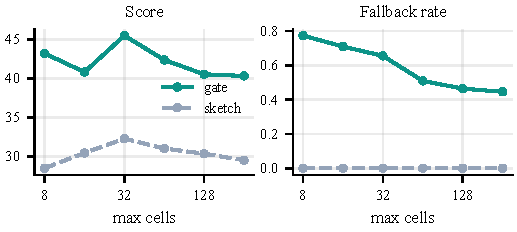
\includegraphics[width=\columnwidth]{figs/sweep_cells.pdf}
\caption{Cell budget sweep (110 questions). The gate holds the score by escalating more often as the budget shrinks.}
\label{fig:sweep}
\end{figure}

\subsection{Long-stream stress test (RQ3, RQ5)}
On the \StressMWords{}M-word stream (Fig.~\ref{fig:stress}), hot memory stays at \StressHotSixtyFour{}~MB with 64 cells
and \StressHotTwoFiftySix{}~MB with 256, while a dense index grows to about \StressDense{}~MB (raw text plus one 384-d
vector per chunk; the raw text alone is \StressText{}~MB). Ingest costs \StressIngest{}~ms per chunk on a CPU. Recall,
however, drops: SketchRAG-gate finds the evidence for \RecSRGate{} of probe questions (256 cells) against \RecDense{}
for dense RAG and \RecBM{} for BM25. Every probe escalates (fallback \StressFb), so SketchRAG behaves like a
two-level router over cold storage: with thousands of unrelated documents sharing a few hundred cells, the cell
centroid is too blunt a key.

\begin{figure}[t]
\centering
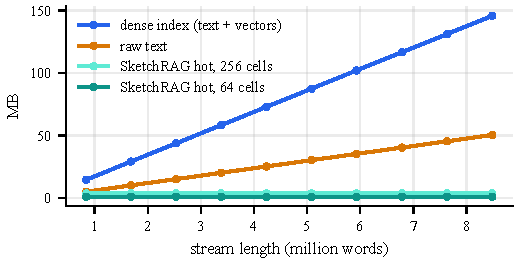
\includegraphics[width=\columnwidth]{figs/stress.pdf}
\caption{Searchable memory vs.\ stream length on the \StressMWords{}M-word stress stream. SketchRAG's hot memory is flat;
cold storage (not shown) grows like the raw text.}
\label{fig:stress}
\end{figure}

\subsection{Comparison with EM-LLM (RQ2)}
\begin{table}[t]
\centering
\caption{Matched comparison with EM-LLM's official code: same base model (Phi-3.5-mini) and the same 120 questions on the 6 LongBench tasks EM-LLM completed.}
\label{tab:emllm}
\setlength{\tabcolsep}{2.6pt}
\footnotesize
\begin{tabular}{lrrrrrrr}
\toprule
System & Qasp & MFQA & HQA & 2WQA & MuSQ & PRet & Avg \\
\midrule
Full context & 39.7 & 41.6 & 38.3 & 35.0 & 11.5 & 60.0 & 37.7 \\
SketchRAG-raw & 34.1 & 40.3 & 56.4 & 18.6 & 24.5 & 43.5 & 36.2 \\
SketchRAG-gate & 40.3 & 47.4 & 47.3 & 16.2 & 20.0 & 37.5 & 34.8 \\
BM25 RAG & 31.4 & 55.0 & 42.4 & 12.1 & 26.7 & 40.0 & 34.6 \\
EM-LLM (official) & 43.2 & 50.9 & 32.9 & 27.7 & 37.5 & 15.0 & 34.5 \\
Dense RAG & 37.5 & 45.0 & 46.3 & 29.8 & 27.7 & 17.5 & 34.0 \\
\bottomrule
\end{tabular}
\end{table}
We ran EM-LLM's official code on two T4 GPUs. The hardware forced changes we record in our repository: weights in fp16
(no bf16 on T4), a smaller GPU block cache, a model split over both GPUs, and disk offload. Its $\infty$-Bench and
NarrativeQA runs exceeded the 29~GB host-RAM limit, so it completed \EMTasks{} of the 9 planned tasks (\EMQ{} questions).
On those, with Phi-3.5-mini as the shared model, SketchRAG-gate and EM-LLM are within a point (\EMGate{} vs.\ \EMLLM{},
Table~\ref{tab:emllm}), with full context highest (\EMFull{}). SketchRAG needs one generation per question rather than
streaming the whole document through the model. EM-LLM ran in fp16 while our Phi-3.5 is Ollama's quantised build, so
the comparison is on the same questions, not an identical model.

\section{Discussion}
\textbf{RQ1.} Extractive streaming summaries preserve topical content but lose exact facts; the raw text they point to
is what recovers them. \textbf{RQ2.} With the gate, SketchRAG beats full context, dense RAG, SARA-lite and AMBER-lite at
the lowest context cost and matches EM-LLM on a shared model, but BM25 remains stronger and multi-hop questions remain
weak. \textbf{RQ3.} Within a document, the budget can shrink to 8--32 cells without losing accuracy because the gate
compensates; across an 8.5M-word stream, memory stays flat but recall falls. \textbf{RQ4.} A deterministic
error-bound gate decides well when the summary is insufficient; a 7B model asked to decide for itself does not.
\textbf{RQ5.} The frozen configuration (64 cells, width 512, two raw chunks per escalated cell) is the best balance we
found; raw pointers must not be cut.

\textbf{Limitations.} The hot memory is bounded but cold storage is not; only the \sys{sketch} policy is bounded end to
end. SARA-lite and AMBER-lite are re-implementations on a shared LLM, not reproductions, and EM-LLM ran at reduced scale.
Answer recall is a string-containment proxy rather than recall against annotated evidence. We use one 7B model and 30
questions per task, so differences under about two points are within noise.

\textbf{Live demonstration.} We also built a web console (Fig.~\ref{fig:demo}) in which an agent monitors a
400k-word feed of LongBench documents, its 256-cell memory updating live, and answers typed questions with a local 3B
model (llama3.2:3b through Ollama on a laptop CPU) while showing each retrieval step, the gate's verdict per cell and the
raw evidence it read.

\begin{figure}[t]
\centering
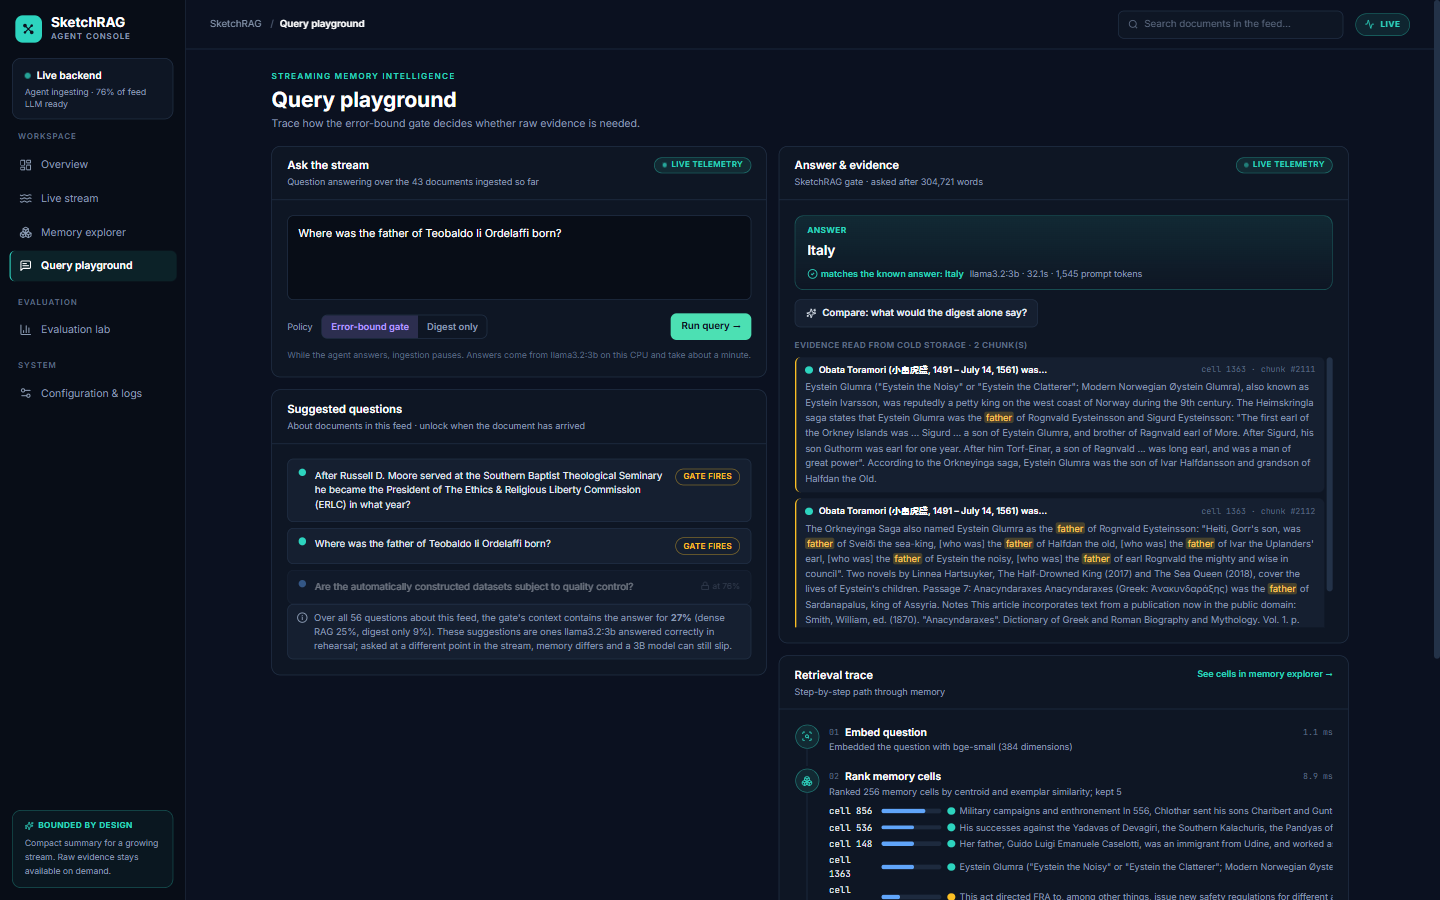
\includegraphics[width=\columnwidth]{figs/demo_query.png}
\caption{Live demo console: a question asked mid-stream, the answer streamed by a local model and checked against the
known answer, the raw chunks read from cold storage, and the retrieval trace (bottom).}
\label{fig:demo}
\end{figure} On that feed the gated context holds the answer for \DemoGate\% of \DemoQ{} questions (dense retrieval \DemoDense\%),
consistent with the stress-test finding.

\section{Conclusion}
SketchRAG shows that classic streaming synopses can serve as a bounded retrieval memory for an LLM agent, provided the
system knows when not to trust them. The Count-Min error bound supplies that knowledge: it escalates exactly the
questions where raw evidence matters and leaves the rest to compact digests, giving competitive accuracy at the lowest
context cost of the systems we tested. The main open problem is recall at stream scale, where a few hundred centroids
are too coarse a key; finer-grained keys, such as a small lexical index over digests or hierarchical cells, and a gate
aware of multi-hop questions are the natural next steps. Code, results and the demo are in our project repository.

\bibliographystyle{IEEEtran}
\bibliography{refs}

\end{document}
